% !TEX root = ../notes_template.tex
\chapter{Movement \& Muscle Testing}\label{chp:muscle_testing}

\section*{Objectives}
\begin{itemize}
  \item Observe global movement patterns and identify the muscles involved in producing or stabilizing those motions.
  \item Apply principles of manual muscle testing (MMT) and muscle length testing (MLT) to assess neuromuscular performance.
  \item Recognize how gross movement dysfunction can inform region-specific muscle testing strategies.
\end{itemize}

\section*{Functional Movement-Based Approach}

A functional movement-based approach uses full-body movement patterns as a top-level screen to identify potential regional or focal problems. This approach is widely applied in all areas of physical therapy practice. For example, physical therapists often observe gait, transfers, breathing patterns, or bed mobility as initial indicators of dysfunction before formulating more specific regional or local hypotheses. 

 Selective Functional Movement Assessment (SFMA)\textsuperscript{\textregistered}\footnote{SFMA\textsuperscript{\textregistered} is a registered trademark of Functional Movement Systems, Inc. Used here for educational reference.} top-tier movements represent one structured example of this strategy. These whole-body screening patterns are used to observe functional mobility and stability/motor control as the first step towards breaking down possible problems (such as joint mobility or stability or motor control problems). Although formal classification is not required at this stage, movements help you begin to see how observed dysfunction can guide muscle testing. Each pattern is performed actively, with the goal of identifying which muscles contribute to or compensate for movement.

\begin{itemize}
  \item \textbf{Cervical Flexion (C-F):} Tuck the chin and bring the head forward to look down, attempting to touch the chin to the chest.
  \item \textbf{Cervical Extension (C-E):} Tilt the head back to look at the ceiling, maintaining a smooth arc of motion.
  \item \textbf{Cervical Rotation (C-R):} Turn the head to the right and left, aiming to align the chin with the shoulder.
  \item \textbf{Upper Extremity Pattern 1 (UE1):} Reach behind the back with the hand, trying to touch the opposite inferior scapular angle (medial rotation, extension, and adduction).
  \item \textbf{Upper Extremity Pattern 2 (UE2):} Reach behind the head with the hand, trying to touch the opposite scapular spine (lateral rotation, flexion, and abduction).
  \item \textbf{Multisegmental Flexion (MSF):} From standing, bend forward to touch the toes with the knees extended, keeping movement smooth through the lumbar, thoracic, and cervical spine.
  \item \textbf{Multisegmental Extension (MSE):} Lean back with arms overhead, extending through the hips, lumbar spine, and shoulders.
  \item \textbf{Multisegmental Rotation (MSR):} Rotate the head, shoulders, and trunk to one side while the feet are planted.
  \item \textbf{Single-Leg Stance (SLS):} Stand on one leg for 10 seconds with arms at the sides and without excessive sway or upper body compensation.
  \item \textbf{Arms Down Deep Squat (DS):} Perform a full bodyweight squat with heels on the floor, arms down and head and chest upright.
\end{itemize}

These movement patterns provide a functional lens for hypothesizing which muscle groups may be short, weak, overactive, or under-recruited. They serve as an entry point for selecting more targeted manual muscle testing (MMT) and muscle length testing (MLT).

It is important to note that any hypothesis drawn from a top-tier (functional) movement should eventually be expanded to include considerations of bone and joint structure - topics you will be exploring this semester in the Osteology \& Arthrology Lab with Dr. DeBaets. As the semester progresses and you become fluent in those concepts, we will periodically incorporate them into this lab to help you begin integrating your anatomical and biomechanical reasoning.

\subsubsection*{Muscle Length, Tension, and Multiarticular Complexity}

Muscles that cross more than one joint present unique clinical challenges and opportunities for insight. These multiarticular muscles are subject to both \textbf{active} and \textbf{passive insufficiency}, which reflect the physiological tension properties of muscles during movement.

\begin{itemize}
  \item \textbf{Active insufficiency} occurs when a muscle is too shortened across multiple joints to generate effective force.
  \item \textbf{Passive insufficiency} occurs when a muscle resists being stretched across multiple joints, limiting the available movement.
\end{itemize}

These principles influence not only how we move, but also how we assess motion, strength, and length. They form the basis for understanding why muscle function must be interpreted in context.

\begin{labactivitybox}
\textbf{Activity: Functional Movement Approach}

Perform each SFMA Top Tier movement and identify, by general synergist groups, the primary muscles responsible for generating and stabilizing the motion. Briefly discuss which muscles (or groups) may be:

\begin{itemize}
  \item Shortened and restricting range
  \item Weak or underactive
  \item Overactive and compensatory
\end{itemize}

\textit{Note:} Dysfunction in movement patterns can arise from a range of causes—including joint restriction, motor control deficits, fascial restrictions, or behavioral factors. In this lab, the focus is specifically on neuromuscular contributions, with an emphasis on reasoning through strength and length impairments.

Use this analysis to generate hypotheses about muscles that may require targeted manual muscle testing (MMT) or muscle length testing (MLT).
\end{labactivitybox}

\begin{tcolorbox}[colback=gray!5, colframe=black, title=Clarifying Movement \& Motion in This Course]

In this course, we draw a practical distinction between \textbf{movement} and \textbf{motion}, rooted loosely in terminology from physics and biomechanics:

\begin{itemize}
  \item \textbf{Motion} is a broad term describing any change in position over time. In biomechanics, this includes both angular and linear displacement, regardless of intent, control, or cause. Clinically, we use “motion” to describe what is observed: the displacement or behavior of a region during activity, including compensations or postural shifts.

  \item \textbf{Movement} is used more narrowly to describe purposeful, controlled osteokinematic actions—like hip abduction or shoulder flexion—produced by muscular effort and typically evaluated with MMT or muscle length tests.
\end{itemize}

\textit{Example:} During arm elevation, scapular upward rotation is a movement—an intentional action associated with specific muscles. In contrast, scapular anterior tipping is a motion—an observed behavior that may reflect imbalance or compensation, but isn’t directly testable or assigned to a primary mover.

This conceptual distinction isn’t universal, but it helps us separate what we observe from what we test. Arthrokinematic joint motions (glide, roll, spin) are addressed in the Osteology \& Arthrology lab and lie outside the direct scope of this course.

By adopting this language, we align with principles of \textit{mechanism-neutral reasoning}\footnote{Mintken PE, Derosa C, Little T, et al. (2008). A Model for Standardizing Manipulation Terminology. \textit{JOSPT}, 38(2):A1–A6.}, supporting open clinical interpretation without presupposing causality.

\end{tcolorbox}

\section*{Manual Muscle Testing (MMT)}

\subsection*{Purpose}
MMT is one way to examine a muscle or muscle group’s ability to generate tension under controlled conditions. While it is a valuable tool for identifying weakness, it does not, on its own, determine the source of that weakness—whether muscular, neural, or due to other factors such as pain, motor control, or effort.

\subsection*{Key Concepts}
\begin{itemize}
  \item \textbf{Fixation:} Stabilization should be applied proximal to the test joint to oppose the action of the target muscle.
  \item \textbf{Break Test:} Resistance is applied gradually until the subject can no longer maintain the test position.
  \item \textbf{Resistance:} Should be applied in the midrange—an attempt to optimize both the muscle’s length–tension relationship and its moment arm—as far from the joint as possible without crossing additional joints (to optimize the resistance lever arm).
  \item \textbf{Gross vs. Specific:} Gross screening assesses general regional strength; specific MMT attempts to isolate individual muscles.
  \item \textbf{Muscle Isolation Strategy:} Isolation is approached by selecting a joint position and resistance direction that place the target muscle in mechanical advantage while minimizing the contribution of synergists. Although true isolation is rarely possible, strategic biasing improves test specificity.
\end{itemize}

\subsubsection*{Length–Tension and Active Insufficiency in MMT}

Manual muscle testing is most accurate when performed at mid-range length—where the muscle produces peak active force. When a multiarticular muscle is too shortened across joints (e.g., hamstrings during hip extension and knee flexion), it may exhibit \textbf{active insufficiency}, resulting in a false impression of weakness. Understanding this helps clinicians select test positions that isolate strength from joint limitations.

\subsubsection*{Limitations of MMT and the Myth of Isolation}

Manual muscle testing is often framed as a method of 'isolating' individual muscles for strength assessment. In reality, true isolation is nearly impossible due to the synergistic and stabilizing contributions of the surrounding musculature, joint positioning, and motor control strategies. The best MMT offers is a position that biases toward a target muscle under standardized conditions.

Equally important is recognizing what MMT cannot tell us: the cause of a weakness. A weak test does not differentiate whether the problem is muscular (e.g., atrophy, tendon injury), neurological (e.g., nerve root compression), energetics (e.g., disturbance in blood flow), motor control related (e.g., inhibition) or effort related (e.g., pain avoidance or fear). Even when weakness is neurological in origin, the source may lie within the central nervous system (e.g., stroke or spinal cord lesion) or the peripheral nervous system (e.g., nerve root or peripheral nerve dysfunction).


\subsubsection*{Beyond MMT: Complementary Strategies for Neuromuscular Assessment}

To move beyond the limitations of MMT, this lab integrates complementary assessment strategies:

\begin{itemize}
  \item \textbf{Reflex testing} supports differentiation of central vs. peripheral nervous system involvement.
  \item \textbf{Pulse palpation} provides insight into the vascular supply.
  \item \textbf{Rehabilitative Ultrasound Imaging (RUSI)} allows real-time visualization of muscle activation, structure, and symmetry, providing insight into control strategies and patterns of use.
  \item \textbf{Electromyography (EMG)}—previewed later in the program - can directly assess motor unit activation and timing, helping to distinguish between neural and muscular causes.
\end{itemize}

\vspace{1em}
\noindent
\textbf{Neurological Weakness: Upper vs. Lower Motor Neuron Patterns} \\
Weakness of neurological origin can result from upper motor neuron (UMN) or lower motor neuron (LMN) lesions. UMN lesions originate in the brain or spinal cord and are often accompanied by spasticity, increased tone, and hyperreflexia. LMN lesions occur at the nerve root or peripheral nerve level and are characterized by flaccid weakness, hyporeflexia, muscle atrophy, and fasciculations. MMT cannot distinguish between these presentations on its own, but when interpreted alongside reflex testing and tone observation, it contributes to differential diagnosis.

When interpreted in isolation, MMT is simply a measure of force production under standardized resistance. Its value comes from integration: Correlating movement patterns, reflexes, muscle tone, imaging, and neurovascular understanding to determine why a muscle is weak, not just whether it is.

Therefore, it is critical to interpret the strength findings within a functional context. A strong MMT result does not guarantee that the intended muscle is functioning optimally, and a weak result does not always mean true muscle pathology. Compensation strategies, altered motor control, and joint positioning all influence the outcome of the test.

MMT should be viewed as a valuable but limited tool, one that generates hypotheses rather than definitive conclusions. Its strength lies in its integration with movement observation, palpation, and clinical reasoning. In certain settings, hand-held dynamometry (HHD) can be used to quantify force output and improve the objectivity and sensitivity of manual testing.

\begin{tcolorbox}[colback=gray!5, colframe=black, title=Testing Muscles Through Movements]
Given the challenges of isolating individual muscles and the fact that muscles can only be tested through their associated osteokinematic actions, manual muscle testing is fundamentally a test of movement. Although testing positions may bias force generation toward a particular muscle, the result always reflects the contribution of synergists, stabilizers, and the quality of motor control.

Throughout this manual, muscles are organized and tested based on the movements they produce. This supports the clinical reasoning rooted in function and reinforces that strength assessments should be interpreted in the context of movement systems, not isolated tissues.
\end{tcolorbox}

\subsection*{Grading}
Manual muscle testing is graded on an ordinal scale of 0-5, with intermediate scores (e.g., 3 +, 4-) used to capture nuances in resistance tolerance, range of motion, and functional relevance. The grading reflects the patient's ability to hold or move against gravity and manual resistance in a standardized position.

\medskip
\noindent
\textit{Reminder:} While MMT is useful to detect weakness, it does not determine the cause of that weakness alone. Reduced force production may reflect muscular limitations, neurological impairments, altered motor control, pain inhibition, or suboptimal effort. Grading should always be interpreted within the broader clinical context.

\begin{table}[H]
\centering
\begin{tabular}{|c|c|p{9cm}|}
\hline
\textbf{Grade} & \textbf{Score} & \textbf{Description} \\
\hline
Normal & 5/5 & Full ROM against gravity with maximal resistance \\
\hline
Good + & 4+/5 & Full ROM against gravity with moderate to strong resistance \\
\hline
Good & 4/5 & Full ROM against gravity with moderate resistance \\
\hline
Good – & 4-/5 & Full ROM against gravity with slight to moderate resistance \\
\hline
Fair + & 3+/5 & Full ROM against gravity with minimal resistance \\
\hline
Fair & 3/5 & Full ROM against gravity but breaks with any resistance \\
\hline
Fair – & 3-/5 & At least 50\% ROM against gravity but not full range \\
\hline
Poor + & 2+/5 & Partial ROM against gravity \textit{or} full ROM in gravity-eliminated position with some resistance \\
\hline
Poor & 2/5 & Full ROM in gravity-eliminated position with no resistance \\
\hline
Poor – & 2-/5 & Partial ROM in gravity-eliminated position \\
\hline
Trace & 1/5 & Palpable contraction with no visible movement \\
\hline
Zero & 0/5 & No palpable contraction \\
\hline
\end{tabular}
\caption{Manual Muscle Testing Grading Scale}
\end{table}

\subsection*{Augmented MMT: Hand-Held Dynamometry}

To overcome some of the limitations of traditional MMT grading, force transducers such as hand-held dynamometers (HHDs) can be used to quantify muscle force. These tools allow the clinician to move from a subjective ordinal scale to an objective, continuous measurement of force output.

\begin{itemize}
  \item Objective, quantifiable measurement of force (typically in Newtons or kilograms).
  \item Reliable comparisons across limbs, sessions, or test positions.
  \item Greater sensitivity to small changes in strength over time.
\end{itemize}

In this lab, students will be introduced to the \textbf{Lafayette 01165A Hand-Held Dynamometer}, which provides real-time digital readouts of peak force and hold durations. This instrument supports standardized resistance testing across muscle groups and will be used to supplement traditional MMT procedures.

\begin{figure}[H]
  \centering
  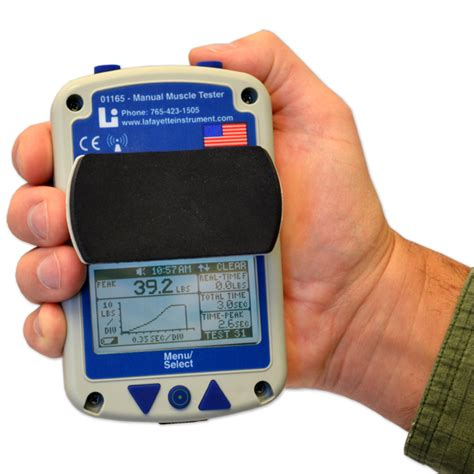
\includegraphics[width=0.4\textwidth]{figure/lafayette_01165a.jpeg}
  \caption{Lafayette 01165A Hand-Held Dynamometer}
  \label{fig:lafayette_hhd}
\end{figure}

Though not universally available in all clinical settings, hand-held dynamometry represents an evidence-informed extension of manual muscle testing. It is particularly useful for documenting progress, informing prognosis, and supporting return-to-activity decisions.

\begin{labactivitybox}
\textbf{Activity: MMT Application Across Planes and Conditions}

You will perform focused testing on two assigned motions:

\begin{itemize}
  \item \textbf{Shoulder abduction} (frontal plane)
  \item \textbf{Hip flexion} (sagittal plane)
\end{itemize}

For each movement, perform the following:

\begin{enumerate}
  \item Position your partner for a gravity-resisted MMT.
  \item Apply a standard \textbf{break test}, observing stabilization and effort.
  \item Repeat the test using the \textbf{Lafayette 01165A Hand-Held Dynamometer} to measure peak force.
  \item Reposition your partner for a \textbf{gravity-eliminated} MMT and reassess the motion.
\end{enumerate}

\textit{Record:}
\begin{itemize}
  \item Which muscles are primarily responsible for producing the movement?
  \item Which test position best allowed you to observe the muscle’s contribution?
  \item How did the resistance application and observed strength differ across test conditions?
  \item What were the practical challenges of using the dynamometer?
  \item Compare performance between the two movements. Were differences more pronounced in break test, gravity-eliminated testing, or HHD force output?
  \item \textbf{Note:} In future labs, you’ll also be responsible for identifying each muscle’s peripheral nerve and most common spinal root(s); as well as how the stabilizers and muscle length of antagonists can influence test results. Use this opportunity to start developing that habit of reasoning.
\end{itemize}
\end{labactivitybox}

\section*{Muscle Length Testing (MLT)}

\subsection*{Purpose}
Muscle length testing is used to determine whether a muscle (including its surrounding connective tissue) can lengthen sufficiently to allow normal joint motion and posture. It helps identify if a muscle is functionally \textbf{limited} (shortened), \textbf{normal}, or \textbf{excessive} (over-lengthened). A shortened muscle may restrict motion, contribute to stiffness, or drive compensatory movement patterns. 

\subsection*{Conceptual Basis}

Muscle length is typically assessed by evaluating the range of motion (ROM) permitted at the joint and reasoning about possible causes if ROM is reduced. Muscle length is one possible reason for reduced ROM (you'll review others in the Osteology \& Arthrology Lab). While this is often expressed in degrees of joint motion, it reflects the extensibility and resting tension of the muscle-tendon unit, not just joint mechanics. Muscle length limitations are particularly common in muscles that lengthen across more than one joint.

\subsubsection*{Passive Insufficiency and Length Testing}

Many special tests for muscle length target multiarticular muscles because of the clear influence of \textbf{passive insufficiency}\footnote{See Chapter 3 of \textit{Clinical Physiology: A Muscle-Centered Approach} for a detailed explanation of passive insufficiency and the length–tension properties of muscle-tendon units.}. This occurs when a muscle cannot lengthen enough to allow acceptable joint excursion at all of the joints crossed by the muscle, such as the hamstrings during combined hip flexion and knee extension. Recognizing passive insufficiency is essential for interpreting muscle length in functional movement.

\subsection*{Testing Procedure}

\begin{itemize}
  \item \textbf{Patient Positioning:} Choose a position—supine, prone, side-lying, or seated—that best exposes the muscle to be lengthened while minimizing compensatory movement.

  \item \textbf{Order of Lengthening:} To assess muscle length, position the patient so that the muscle is elongated across all the joints it spans. This typically involves moving the joints in the direction opposite to the muscle’s action—starting with the joint closest to the muscle’s origin and progressing toward the joint nearest its insertion. For example, when testing the hamstrings, begin by flexing the hip and then extending the knee. This sequence ensures a controlled, functional stretch of the muscle-tendon unit.

  \item \textbf{Tissue Resistance Points:}
    \begin{itemize}
      \item \textbf{R1 (First Resistance):} The first perceptible increase in tissue tension, which may limit available motion or alter control.
      \item \textbf{R2 (Second Resistance):} The end of available range, marked by a firm stop, compensatory motion, or discomfort.
    \end{itemize}

  \item \textbf{Observation:} Monitor for substitution patterns such as pelvic tilt, spinal shift, scapular elevation, or altered joint mechanics, which suggest compensation or movement limitation.

  \item \textbf{Determination:} Based on range, tissue resistance, and symmetry with the opposite side, classify the muscle length as \textbf{Limited}, \textbf{Normal}, or \textbf{Excessive}.
\end{itemize}

\subsection*{Clinical Context}
MLT findings should always be interpreted in the context of functional movement patterns. A muscle that appears long may in fact be under-recruited or inhibited; one that is short may be overactive or stiff. MLT, like MMT, is hypothesis-generating and should be integrated with movement observation and neurovascular examination.

\begin{labactivitybox}
\textbf{Activity: Rectus Femoris Muscle Length Testing – Modified Thomas Test}

This activity guides you through assessment of the rectus femoris using a proximal-to-distal joint sequencing strategy, consistent with standard testing logic.

\textbf{Procedure:}
\begin{itemize}
  \item Position the patient supine at the edge of the table, holding one knee to the chest.
  \item Allow the test leg to drop into hip extension.
  \item Passively flex the knee to assess length, observing for R1 (initial resistance), R2 (firm end-range), and any compensations (e.g., pelvic tilt).
\end{itemize}

\textbf{Clinical Note:} This test follows the typical “proximal to distal” sequence (hip extension then knee flexion), aligning with common instructional frameworks.

\textit{Record:}
\begin{itemize}
  \item When did R1 and R2 occur?
  \item What compensations were observed?
  \item Classify length as \textbf{Limited}, \textbf{Normal}, or \textbf{Excessive}.
  \item Was the result symmetrical between limbs?
\end{itemize}
\end{labactivitybox}

\begin{labactivitybox}
\textbf{Activity: Hamstring Muscle Length Testing – Straight Leg Raise (SLR)}

This activity evaluates hamstring length using the passive straight leg raise. This common clinical test reverses the typical joint sequencing heuristic.

\textbf{Procedure:}
\begin{itemize}
  \item Position the patient supine with the non-test leg flat.
  \item Passively flex the hip with the test knee extended.
  \item Observe for R1, R2, and any compensatory movements (e.g., posterior pelvic tilt, lumbar flattening).
\end{itemize}

\textbf{Clinical Note:} Unlike standard sequencing, this test proceeds distal-to-proximal (knee extended, then hip flexed). Consider how this reversal influences your interpretation of passive insufficiency.

\textit{Record:}
\begin{itemize}
  \item When did R1 and R2 occur?
  \item What compensations were observed?
  \item Classify length as \textbf{Limited}, \textbf{Normal}, or \textbf{Excessive}.
  \item Was the result symmetrical between limbs?
  \item \textbf{Reflection:} How might you modify this test to follow a proximal-to-distal sequence? Would that improve or hinder interpretation?
\end{itemize}
\end{labactivitybox}

\section*{Clinical Integration}

\begin{itemize}
  \item How does functional movement screening (e.g., SFMA Top Tier) inform your selection of specific MMT or MLT procedures?
  \item What are the limitations of MMT and MLT when interpreted in isolation? How do you begin to reason through cause vs. compensation?
  \item Where did you observe passive or active insufficiency? How did it affect your interpretation of muscle function?
  \item How might the results of these tests guide further investigation (e.g., reflex testing, palpation, RUSI)?
\end{itemize}

\section*{Next Steps}

\begin{itemize}
  \item Review the principles of manual muscle and length testing, with attention to test positioning, stabilization, and resistance application.
  \item Practice MMT and MLT procedures for the hamstrings and rectus femoris during Open Lab or Recitation as review of the underlying principles (you'll be doing these tests again when we get to pelvis/hip).
  \item Begin reviewing innervation (peripheral nerve and nerve root) for the muscles you tested, as this will be central to Week 2.
  \item Preview Chapter 3 in \textit{Clinical Physiology: A Muscle-Centered Approach} to reinforce your understanding of the length–tension relationship and insufficiency patterns (we'll be covering it next week in Clinical Physiology anyway).
\end{itemize}

\section*{Checklist Summary}

\begin{itemize}
  \item [$\square$] Performed and interpreted SFMA Top Tier patterns, with identification of major muscle contributors.
  \item [$\square$] Conducted gravity-resisted MMT for hip flexion and shoulder abduction, with break test and HHD measurement.
  \item [$\square$] Performed gravity-eliminated MMT for one assigned motion, using appropriate positioning and stabilization.
  \item [$\square$] Documented primary movers, observed strength, and compensation patterns for MMT scenarios.
  \item [$\square$] Conducted modified Thomas test and interpreted rectus femoris length, including R1, R2, and observed compensations.
  \item [$\square$] Conducted straight leg raise (SLR) for hamstrings, with R1, R2, and interpretation of sequencing and compensations.
\end{itemize}
